\chapter{第二部分}
\section{问题概述}
%
%%对问题的直观描述
%
%
%对项目已有代码的阅读和理解
%
%
%解决问题的思路和想法
%
该部分包含第5、6小题。

该部分所要解决的搜索问题是让吃豆人遍历迷宫的四个角落。题目要求我们先对该问题进行形式化,然后给出相应的具有一致性的启发式函数。

这一搜索问题的状态除了吃豆人当前位置外,还需要以某种方式记录下目前为止遍历了哪些角落,以便进行目标检验。因此和第一部分中的问题相比,
该搜索问题的转移函数等部分还需额外处理状态中新增的记录。

由于该问题中需要遍历的位置是固定的四个角落,因此可以在忽视墙壁的条件下, 求出的遍历四个角所需要的最小的曼哈顿距离便可以作为启发式函数。
\section{算法设计}
%
%用自己的语言描述解决问题所使用的算法的原理及功能,设计思路和算法流程图
%
由于遍历四个角时,必会先达到其中一个角。而当忽视墙壁时,从任意一个角出发,遍历其他三个角所需要的最短路径显然是一样的,均为宽和高之和,再加上两者中较小的一个。
因此,从迷宫中的任意一点出发,不断朝着最近的一个未遍历过的角落前进便可以得到最短的总距离。而由于这是在放松限制条件下得到的最优解,所以它的长度可以作为实际问题的启发式函数。

\begin{procedure}
    \KwOut{cost}
    \SetKwFunction{manhattanDistance}{manhattanDistance}
    \SetKw{in}{in}
    cost = 0\;
    \While(\tcp*[h]{还有未遍历的位置}){goals}
    {
        nearestDest = inf\;
        nearest = None\;
        \ForEach{goal \in goals}
        {
            \If{manhattanDistance(position,goal)<nearestDest}
            {
                nearestDest = manhattanDistance(position,goal)\;
                nearest = goal
            }
        }
        cost += nearestDest\;
        goals.remove(nearest)\;
        position = nearest\tcp*[h]{更新为最近目标}\;
    }
    \KwRet{cost}
    \caption{greedy(position,goals)}
\end{procedure}

要证明一个启发式函数是一致的,只需证明对于任意一个动作,前后状态对应的启发式函数值的减少量不大于该动作的代价即可。而当忽视墙壁时,由于该启发式函数值可以分为两部分:
到达最近的一个角落所需的曼哈顿距离,以及从这个角落出发遍历其他角落所需的最小曼哈顿距离之和,而后者并不会因为吃豆人的动作发生改变,同时前者的减少量不大于动作的代价。
所以这一启发式函数是一致的。
\section{算法实现}
%
%在算法原理的基础上,结合代码,讲述算法的实现细节、和兴函数、模块输入输出,数据结构定义等内容
%
由于我的generalGraphSearch中将状态作为reached表的键,所以要求状态所使用的类型是可以散列的。同时,我所设计的启发式函数在计算时需要不断更新状态的遍历记录。
因此,我采用整数来存储遍历记录。取整数的低4位,分别代表4个角落,为1则表示还未遍历,否则表示已遍历。

在CornersProblem类中,\_\_init\_\_和getCostOfAction方法无需进行修改。下面给出修改后的其他方法

\begin{lstlisting}
def getStartState(self):
    # 用01串来记录是否已经达到各个位置,这样方便改动,且是hashable
    return self.startingPosition, (1 << len(self.corners)) - 1
\end{lstlisting}

\begin{lstlisting}[emph={[3]parent,pathCost,problem,heuristic,state},emphstyle={[3]\color{vscode_parametercolor}},emph={[4]SearchProblem,Callable,Node,Actions,Reached,Any},emphstyle={[4]\color{vscode_classcolor}}]
def isGoalState(self, state: Any):
    return not state[1]  # 存储历史的整数为0,即各位为0
\end{lstlisting}

\begin{lstlisting}[emph={[3]parent,pathCost,problem,heuristic,state},emphstyle={[3]\color{vscode_parametercolor}},emph={[4]SearchProblem,Callable,Node,Reached,Any},emphstyle={[4]\color{vscode_classcolor}}]
Successors = namedtuple('Successors', ('cornerProblemState', 'action', 'pathCost'))
def getSuccessors(self, state: Any):
    successors = []
    for action in [Directions.NORTH, Directions.SOUTH, Directions.EAST, Directions.WEST]:
        x, y = state[0]
        goals = state[1]
        dx, dy = Actions.directionToVector(action)
        nextx, nexty = int(x + dx), int(y + dy)
        if not self.walls[nextx][nexty]:
            nextpos = (nextx, nexty)
            remains = goals
            if nextpos in self.corners:
                index = self.corners.index(nextpos)
                remains = remains ^ (1 << index)  # 取反
            successors.append(Successors((nextpos, remains), action, 1))
    self._expanded += 1  # DO NOT CHANGE
    return successors
\end{lstlisting}

下面给出的是启发式函数的实现。
\begin{lstlisting}[emph={[3]parent,pathCost,problem,heuristic,state,goals,position},emphstyle={[3]\color{vscode_parametercolor}},emph={[4]SearchProblem,Callable,Node,Reached,Any},emphstyle={[4]\color{vscode_classcolor}}]
def greedy(position: tuple, goals: List[tuple]) -> float:
    cost = 0
    while goals:
        nearestDest = inf
        nearest = None
        for goal in goals:
            if manhattanDistance(position, goal) < nearestDest:
                nearestDest = manhattanDistance(position, goal)
                nearest = goal
        cost += nearestDest
        goals.remove(nearest)
        position = nearest
    return cost
\end{lstlisting}
\begin{lstlisting}[emph={[3]parent,pathCost,problem,heuristic,state,goals,position},emphstyle={[3]\color{vscode_parametercolor}},emph={[4]SearchProblem,Callable,Node,Reached,Any},emphstyle={[4]\color{vscode_classcolor}}]
def cornersHeuristic(state: Any, problem: CornersProblem):
    corners = problem.corners  # These are the corner coordinates
    walls = problem.walls  # These are the walls of the maze, as a Grid (game.py)
    if not state[1]:
        return 0
    remains = [corner for index, corner in enumerate(corners) if 1 & (state[1] >> index)]  # 获取还未遍历到的角落
    return greedy(state[0], remains)
\end{lstlisting}
\section{实验结果}
\subsection{Question5}
成功通过本问题的全部测试,实验结果截图见图\ref{q5}。测试用例是一个小型迷宫。
\begin{figure}[htbp]
    \centering
    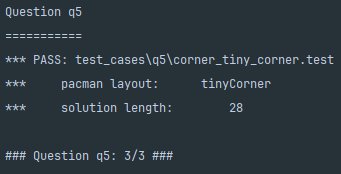
\includegraphics[scale = 0.7]{pic/q5.png}
    \caption{Question5实验结果}\label{q5}
\end{figure}
\subsection{Question6}
成功通过本问题的全部测试,实验结果截图见图\ref{q6}。共有四个测试样例,用于测试所设计的启发式函数是否是一致的。前三个样例为小型迷宫,最后一个样例为中型迷宫。
\begin{figure}[htbp]
    \centering
    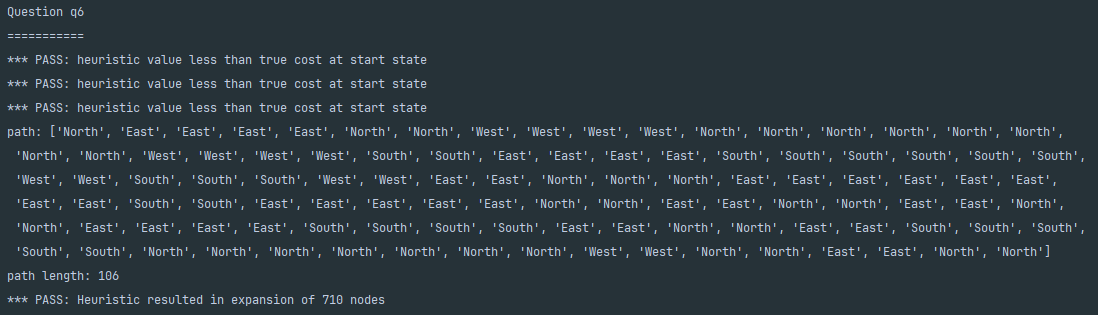
\includegraphics[width = \textwidth]{pic/q6.png}
    \caption{Question6实验结果}\label{q6}
\end{figure}
%
%对试验结果进行详细展示,对每个问题展示测试截图,对于测试用例进行描述说明,对于为通过测试的用例结合自己的算法进行分析,可以结合调试过程进行分析
%
%实验中遇到的问题及解决方案,收获和思考:对算法的理解、优缺点的评价、算法的适用场景
%
